\chapter{解析結果}
本研究は,ゴルフスイングを数値化したデータに,ヒルベルト・ファン変換を適用させ,瞬時周波数領域で解析を行う.
\section{ゴルフスイングの数値化}
ゴルフスイングの数値化は,慣性式モーションキャプチャを使用して行う.
使用するモーションキャプチャは,PERCEPTION NEURON 2.0を使用する.
\begin{figure}
    \begin{center}
        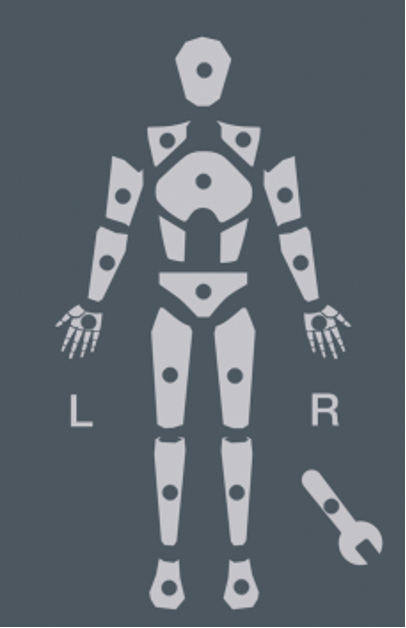
\includegraphics[width=5.0cm]{./images/sensors.png}
        \caption{加速度センサがついている位置}
        \label{sensors}
    \end{center}
\end{figure}
PERCEPTION NEURON 2.0は,図\ref{sensors}のように17点の位置に加速度センサを装着する.
この加速度センサより,推定の位置座標と$x$$y$$z$軸方向の回転角度を時系列にキャプチャする.


\section{被験者情報}

\section{スペクトログラム解析}
\subsection{頸部,左膝モーションのIMF1}
\subsection{頸部,左膝,左腿モーションのIMF4}